\documentclass[12pt]{article}

\pagestyle{empty}
\setlength{\topmargin}{0in}
\setlength{\headheight}{0in}
\setlength{\topsep}{0in}
\setlength{\textheight}{9in}
\setlength{\oddsidemargin}{0in}
\setlength{\evensidemargin}{0in}
\setlength{\textwidth}{6.5in}

\usepackage{palatino,amssymb,amsmath,graphicx}

\newcommand{\real}{{\bf R}}
\newcommand{\vs}[1]{\vspace{#1in}}

\begin{document}

\input epsf.sty

\noindent
{\bf Mathematics 227} \\ 
{\bf Lab 1, Due: September 10, 2018} \\
\bigskip

\noindent
{\bf Instructions:} Complete the following exercises in
groups of 2 or 3 students, but you only need to hand in one report for
your group.  You may write directly on this handout; be sure to
include complete explanations of the work you have done.

\medskip
There is a page of Sage cells available at
{\tt http://gvsu.edu/s/0Ng}

\begin{enumerate}
\item Consider the system of linear equations:
  $$
  \begin{alignedat}{4}
    x & {}+{} & 2y & {}-{} & z & {}={} & 1 \\
    3x & {}+{} & 2y & {}+{} & 2z & {}={} & 7 \\
    -x & & & {}+{} & 4z & {}={} & -3 \\
  \end{alignedat}
  $$
  Write this system as an augmented matrix and use Sage to
  find a description of the solution space.

  \vs{2}

  \newpage
\item Shown below is the traffic pattern in the downtown area of
    a large city.  The figures give the number of cars per hour
    traveling along each road.  Any car that drives into an
    intersection must also leave the intersection.  This means that
    the number of cars entering an intersection in an hour is equal to
    the number of cars leaving the intersection.

    \begin{center}
      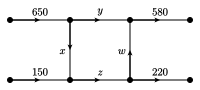
\includegraphics{traffic-a.eps}
    \end{center}

    Write a system of equations for 
    the quantities $x$, $y$, $z$, and $w$
    and describe the set of solutions.  Is there a single solution,
    infinitely many solutions, or no solutions?


    \vs{2}

    Explain why you would expect infinitely many solutions for this
    particular traffic pattern. 

    \vs{1.5}
    What is the smallest amount of traffic flowing through
    $x$?

    \vs{1}
    \newpage
\item A typical problem in thermodynamics is to determine the
  temperature distribution across a thin plate if you know the
  temperature around the boundary.  Assume, for instance, that the
  plate represents a cross section of a metal beam with negligible
  heat flow in the direction perpendicular to the plate.  Let $T_1,
  \ldots, T_6$ be the temperatures at the six nodes inside the beam.
  The temperature at a node is approximately the average of the four
  nearest nodes: for instance,
  $$ T_1 = (10 + 15 + T_2 + T_4)/4 ~~~\hbox{ or } ~~~4T_1 - T_2 - T_4 =
  25.$$
  
  \begin{center}
    \includegraphics{heat.eps}
  \end{center}
  
  In the real world, the approximation becomes better the closer the
  points are together or as we add more and more into the grid.
  
  Set up a system of linear equations to find the temperature inside
  the plate.
  
  \vs{2}
  
  Solve your equations to find the temperatures
  inside the plate.

  {\em Helpful Sage hint:}  If you have a matrix
  {\tt B} containing rational entries (e.g. fractions), you can obtain
  a decimal approximation using {\tt B.numerical\_approx(digits=4)}.
  You may, of course, change 4 to any other appropriate value.
  
  \vs{2}

\item This exercise is about balancing chemical reactions.

  Chemists denote a molecule of water as
  $\text{H}_2\text{O}$, which means it is composed of two
  atoms of hydrogen (H) and one atom of oxygen (O).
  The process by which hydrogen is burned is described by the
  chemical reaction
  $$
  x\thinspace \text{H}_2 + y\thinspace\text{O}_2 \to
  z\thinspace \text{H}_2\text{O}
  $$
  This means that $x$ molecules of hydrogen
  $\text{H}_2$ combine with $y$ molecules of
  oxygen $\text{O}_2$ to produce $z$ water molecules.
  The number of hydrogen atoms is the same before and after
  the reaction;  the same is true of the oxygen atoms.

  \medskip
  How many hydrogen atoms are there before the
  reaction?  How many hydrogen atoms are there after the
  reaction?  Find a linear equation in $x$,
  $y$, and $z$ by equating these quantities.

  \vs{1}
  Find a second linear equation in $x$, $y$, and $z$
  by equating the number of
  oxygen atoms before and after the reaction.

  \vs{1}
  Describe the solutions of this linear system.
  Why would you expect infinitely many solutions when balancing a
  chemical reaction?

  \vs{2}
  In this chemical setting, $x$, $y$, and $z$
  should be positive integers.  Find
  the solution where $x$, $y$, and $z$
  are the smallest possible positive integers.

  \vs{1}


  Consider the reaction where potassium permanganate and manganese
  sulfate combine with water to produce manganese dioxide, potassium
  sulfate, and sulfuric acid:
  $$
  x_1\thinspace \mbox{K}\mbox{Mn}\mbox{O}_4 + 
  x_2\thinspace \mbox{Mn}\mbox{S}\mbox{O}_4 + 
  x_3\thinspace \mbox{H}_2\mbox{O} \to
  x_4\thinspace \mbox{Mn}\mbox{O}_2 + 
  x_5\thinspace \mbox{K}_2\mbox{S}\mbox{O}_4 + 
  x_6\thinspace \mbox{H}_2\mbox{S}\mbox{O}_4.
  $$
  As in the previous exercise, find the appropriate values for
  $x_1,x_2,\ldots, x_6$ to balance the chemical reaction.


\end{enumerate}


\end{document}


